% ŠABLONA PRO PSANÍ ZÁVĚREČNÉ STUDIJNÍ PRÁCE
%%%%%%%%%%%%%%%%%%%%%%%%%%%%%%%%%%%%%%%%%%%%
% Autor: Jakub Dokulil (kubadokulil99@gmail.com)
% Tato šablona byla vytvořena tak, aby pomocí ní mohli v systému LaTeX soutěžící sázet své práce a zároveň odpovídala požadavkům na formátování vyplývajícím z wordové šablony umístěné na webu soc.cz.
%
\documentclass[12pt, a4paper,
%oneside,      %% -- odkomentujte, pokud chcete svou práci mít pouze jednostrannou, mezera pro hřbet pak automaticky bude pouze na levé straně
twoside,        %% -- pro oboustranné práce, mezera pro hřbet následně střídá strany.
openright
]{report}

%% Nutné balíčky a nastavení
%%%%%%%%%%%%%%%%%%%%%%%%%%%%

%% Proměnné
\newcommand\obor{INFORMAČNÍ TECHNOLOGIE} %% -- napiš číslo a název tvého oboru
\newcommand\kodOboru{18-20-M/01} %% -- napiš číslo a název tvého oboru
\newcommand\zamereni{se zaměřením na počítačové sítě a programování} %% -- napiš číslo a název tvého oboru
\newcommand\skola{Střední škola průmyslová a umělecká, Opava} %% vyplň název školy
\newcommand\trida{IT4} %% vyplň jméno svého konzultanta
\newcommand\jmenoAutora{Daniel Antoš}  %% vyplň své jméno
\newcommand\skolniRok{2023/24} %% vyplň rok
\newcommand\datumOdevzdani{1. 1. 2024} %% vyplň rok
\newcommand\nazevPrace{Programovací jazyk Ruda} %% vyplň název své práce

\title{\nazevPrace} %% -- Název tvé práce
\author{\jmenoAutora} %% -- tvé jméno
\date{\datumOdevzdani} %% -- rok, kdy píšeš SOČku

%% Proměnné

%% Proměnné
\newcommand\city{Opava} %% vyplň oficiální název města
\newcommand\district{Moravskoslezský kraj} %% vyplň oficiální název kraje
\newcommand\specialization{Obor č. 18: Informatika} %% -- napiš číslo a název tvého oboru
\newcommand\school{ Střední škola průmyslová a umělecká, Praskova 399/8, Opava, 746 01} %% vyplň název školy
\newcommand\consultant{Mgr. Marek Lučný} %% vyplň jméno svého konzultanta
\newcommand\authorName{Daniel Antoš}  %% vyplň své jméno
\newcommand\publicationYear{2024} %% vyplň rok
\newcommand\mainTitle{Programovací jazyk Ruda} %% vyplň název své práce

\usepackage[top=2.5cm, bottom=2.5cm, left=3.5cm, right=1.5cm]{geometry} %% nastaví okraje, left -- vnitřní okraj, right -- vnější okraj

\usepackage[czech]{babel} %% balík babel pro sazbu v češtině
\usepackage[utf8]{inputenc} %% balíky pro kódování textu
\usepackage[T1]{fontenc}
\usepackage{cmap} %% balíček zajišťující, že vytvořené PDF bude prohledávatelné a kopírovatelné

\usepackage{graphicx} %% balík pro vkládání obrázků

\usepackage{subcaption} %% balíček pro vkládání podobrázků

\usepackage{hyperref} %% balíček, který v PDF vytváří odkazy

\linespread{1.25} %% řádkování
\setlength{\parskip}{0.5em} %% odsazení mezi odstavci


\usepackage[pagestyles]{titlesec} %% balíček pro úpravu stylu kapitol a sekcí
\titleformat{\chapter}[block]{\scshape\bfseries\LARGE}{\thechapter}{10pt}{\vspace{0pt}}[\vspace{-22pt}]
\titleformat{\section}[block]{\scshape\bfseries\Large}{\thesection}{10pt}{\vspace{0pt}}
\titleformat{\subsection}[block]{\bfseries\large}{\thesubsection}{10pt}{\vspace{0pt}}


\usepackage{tocloft} % Balíček umožní přizpůsobit vzhled tabulky obsahu
\setlength{\cftbeforechapskip}{0pt}  % Menší rozestup pro kapitoly
\setlength{\cftbeforesecskip}{0pt}   % Menší rozestup pro sekce

\setcounter{secnumdepth}{2}
\setcounter{tocdepth}{1}
\usepackage{fancyhdr}
\pagestyle{fancy}
\fancyhf{}
\renewcommand{\headrulewidth}{0pt}
\fancyfoot[C]{\thepage}

\usepackage{booktabs}

\usepackage{url}

%% Balíčky co se můžou hodit :) 
%%%%%%%%%%%%%%%%%%%%%%%%%%%%%%%

\usepackage{pdfpages} %% Balíček umožňující vkládat stránky z PDF souborů, 

\usepackage{upgreek} %% Balíček pro sazbu stojatých řeckých písmen, třeba u jednotky mikrometr. Například stojaté mí: \upmu, stojaté pí: \uppi

\usepackage{amsmath}    %% Balíčky amsmath a amsfonts 
\usepackage{amsfonts}   %% pro sazbu matematických symbolů
\usepackage{esint}     %% pro sazbu různých integrálů (např \oiint)
\usepackage{mathrsfs}
\usepackage{helvet} % Helvet font
\usepackage{mathptmx} % Times New Roman
\usepackage{Oswald} % Oswald font


%% makra pro sazbu matematiky
\newcommand{\dif}{\mathrm{d}} %% makro pro sazbu diferenciálu, místo toho
%% abych musel psát '\mathrm{d}' mi stačí napsat '\dif' což je mnohem 
%% kratší a mohu si tak usnadnit práci

\let\oldchapter\chapter
\renewcommand{\chapter}{
	\clearpage
	\pagestyle{fancy}
	\oldchapter
}

\renewcommand\bibname{Seznam použitých zdrojů}


\usepackage{listings}
\usepackage{xcolor}

\renewcommand{\lstlistingname}{Kód}% Listing -> Algorithm
\renewcommand{\lstlistlistingname}{Seznam programových kódů}% List of Listings -> List of Algorithms

%% Definice 
\lstdefinelanguage{JavaScript}{
	morekeywords=[1]{break, continue, delete, else, for, function, if, in,
		new, return, this, typeof, var, void, while, with},
	% Literals, primitive types, and reference types.
	morekeywords=[2]{false, null, true, boolean, number, undefined,
		Array, Boolean, Date, Math, Number, String, Object},
	% Built-ins.
	morekeywords=[3]{eval, parseInt, parseFloat, escape, unescape},
	sensitive,
	morecomment=[s]{/*}{*/},
	morecomment=[l]//,
	morecomment=[s]{/**}{*/}, % JavaDoc style comments
	morestring=[b]',
	morestring=[b]"
}[keywords, comments, strings]


\lstdefinelanguage[ECMAScript2015]{JavaScript}[]{JavaScript}{
	morekeywords=[1]{await, async, case, catch, class, const, default, do,
		enum, export, extends, finally, from, implements, import, instanceof,
		let, static, super, switch, throw, try},
	morestring=[b]` % Interpolation strings.
}

\lstalias[]{ES6}[ECMAScript2015]{JavaScript}

% Nastavení barev
% Requires package: color.
\definecolor{mediumgray}{rgb}{0.3, 0.4, 0.4}
\definecolor{mediumblue}{rgb}{0.0, 0.0, 0.8}
\definecolor{forestgreen}{rgb}{0.13, 0.55, 0.13}
\definecolor{darkviolet}{rgb}{0.58, 0.0, 0.83}
\definecolor{royalblue}{rgb}{0.25, 0.41, 0.88}
\definecolor{crimson}{rgb}{0.86, 0.8, 0.24}

% Nastavení pro Python
\lstdefinestyle{Python}{
	language=Python,
	backgroundcolor=\color{white},
	basicstyle=\ttfamily,
	breakatwhitespace=false,
	breaklines=false,
	captionpos=b,
	columns=fullflexible,
	commentstyle=\color{mediumgray}\upshape,
	emph={},
	emphstyle=\color{crimson},
	extendedchars=true,  % requires inputenc
	fontadjust=true,
	frame=single,
	identifierstyle=\color{black},
	keepspaces=true,
	keywordstyle=\color{mediumblue},
	keywordstyle={[2]\color{darkviolet}},
	keywordstyle={[3]\color{royalblue}},
	literate=%
	{á}{{\'a}}1 {č}{{\v{c}}}1 {ď}{{\v{d}}}1 {é}{{\'e}}1 {ě}{{\v{e}}}1
	{í}{{\'i}}1 {ň}{{\v{n}}}1 {ó}{{\'o}}1 {ř}{{\v{r}}}1 {š}{{\v{s}}}1
	{ť}{{\v{t}}}1 {ú}{{\'u}}1 {ů}{{\r{u}}}1 {ý}{{\'y}}1 {ž}{{\v{z}}}1,		
	numbers=left,
	numbersep=5pt,
	numberstyle=\tiny\color{black},
	rulecolor=\color{black},
	showlines=true,
	showspaces=false,
	showstringspaces=false,
	showtabs=false,
	stringstyle=\color{forestgreen},
	tabsize=2,
	title=\lstname,
	upquote=true  % requires textcomp	
}


\lstdefinestyle{JSES6Base}{
	backgroundcolor=\color{white},
	basicstyle=\ttfamily,
	breakatwhitespace=false,
	breaklines=false,
	captionpos=b,
	columns=fullflexible,
	commentstyle=\color{mediumgray}\upshape,
	emph={},
	emphstyle=\color{crimson},
	extendedchars=true,  % requires inputenc
	fontadjust=true,
	frame=single,
	identifierstyle=\color{black},
	keepspaces=true,
	keywordstyle=\color{mediumblue},
	keywordstyle={[2]\color{darkviolet}},
	keywordstyle={[3]\color{royalblue}},
 literate=%
{á}{{\'a}}1 {č}{{\v{c}}}1 {ď}{{\v{d}}}1 {é}{{\'e}}1 {ě}{{\v{e}}}1
{í}{{\'i}}1 {ň}{{\v{n}}}1 {ó}{{\'o}}1 {ř}{{\v{r}}}1 {š}{{\v{s}}}1
{ť}{{\v{t}}}1 {ú}{{\'u}}1 {ů}{{\r{u}}}1 {ý}{{\'y}}1 {ž}{{\v{z}}}1,		
	numbers=left,
	numbersep=5pt,
	numberstyle=\tiny\color{black},
	rulecolor=\color{black},
	showlines=true,
	showspaces=false,
	showstringspaces=false,
	showtabs=false,
	stringstyle=\color{forestgreen},
	tabsize=2,
	title=\lstname,
	upquote=true  % requires textcomp
}

\lstdefinestyle{JavaScript}{
	language=JavaScript,
	style=JSES6Base,
}
\lstdefinestyle{ES6}{
	language=ES6,
	style=JSES6Base
}


%% Bordel pro práci - můžeš smáznout :) 
%%%%%%%%%%%%%%%%%%%

\usepackage{lipsum} %% balíček který píše lipsum (nesmyslný text, který se používá pro kontrolu typografie)


%% Začátek dokumentu
%%%%%%%%%%%%%%%%%%%%
\begin{document}
	
	\pagestyle{empty}
	\pagenumbering{Roman}
	
	\begin{titlepage}
		\bfseries{ %%% písmo na stránce je tučně
			\begin{center}
				\LARGE{STŘEDOŠKOLSKÁ ODBORNÁ ČINNOST}
				
				\vspace{14pt}
				\large{ %%%%
					\specialization
				} %%%%
				
				\vspace{0.2 \textheight}
				
				\LARGE{ %%%%
					\mainTitle
				}%%%%
				
				\begin{figure}[h]
					\centering
					
\includegraphics[width=0.3\linewidth]{image/logo.png} 
				\end{figure}
				
				\vspace{0.2\textheight}
			\end{center}
			
			\noindent\Large{\authorName} 
			
			\noindent\Large{\district \hspace{\stretch{1}}  \city, \publicationYear} 
			
			
		} %%%
	\end{titlepage}
	
	\cleardoublepage
	
	%% Úvodní stránka s informacemi
	{\bfseries %%% písmo na stránce je tučně
		\begin{center}
			\LARGE{STŘEDOŠKOLSKÁ ODBORNÁ ČINNOST}
			
			\vspace{14pt}
			{\large %%%%
				\specialization %% -- napiš číslo a název tvého oboru
			} %%%%
			
			\vspace{0.3 \textheight}
			
			\LARGE{ %%%%
				\mainTitle
			}
			
			\LARGE{ %%%%
				The Ruda programming language
			}%%%%
			
			\vspace{0.24\textheight}
		\end{center}  
	}%%%
	{\Large %%%
		\noindent\textbf{Jméno:} \authorName\\
		\textbf{Škola:} \school\\
		\textbf{Kraj:} \district\\
		\textbf{Konzultant:} \consultant\\
	} %%%
	
	\noindent \city, \publicationYear
	
	\cleardoublepage

	\noindent{\Large{\bfseries{Prohlášení}}}  %% uprav si koncovky podle toho na jaký rod se cítíš, vypadá to pak lépe :) 
	
	\noindent Prohlašuji, že jsem svou práci SOČ vypracoval/a samostatně a použil/a jsem pouze prameny a literaturu uvedené v seznamu bibliografických záznamů.
	
	\noindent Prohlašuji, že tištěná verze a elektronická verze soutěžní práce SOČ jsou shodné. 
	
	\noindent Nemám závažný důvod proti zpřístupňování této práce v souladu se zákonem č. 121/2000 Sb., o právu autorském, o právech souvisejících s právem autorským a o změně některých zákonů (autorský zákon) ve znění pozdějších předpisů. 
	
	\vspace{24 pt}
	
	\noindent V Branticích dne 11. dubna 2024 \dotfill{}\hspace{\stretch{0.5}} 
	
	\hspace{8cm} \authorName
	
	\cleardoublepage
	
	%% Stránka obsahující abstrakt (anotaci)
	%%%%%%%%%%%%%%%%%%%%%%%%%%%%%%%%%%%%%%%%%%%%%%%%%%%%%%%%	
	
	%% Abstrakt v češtině
	%%%%%%%%%%%%%%%%%%%%%%%%%%%%
		\noindent{\Large{\bfseries{Anotace}\\}}
		\noindent 
		Ruda je programovací jazyk zaměřený na rychlé a snadné prototypování aplikací, umožňující vývojářům rychle testovat nápady bez zbytečné složitosti. Kompiluje se do systémově nezávislého binárního formátu pro rychlé spuštění pomocí Ruda VM. Jednoduchá syntaxe a vestavěné nástroje usnadňují vytváření prototypů.
		
		\vspace{18pt}
		
		\noindent{\large{\bfseries{Klíčová slova}}}
		
		\noindent Programovací jazyk, kompilace, parser, interpret
		
		\vspace{18pt}
		
		\noindent{\Large{\bfseries{Annotation}}}
		
		\noindent 
		Ruda is a programming language focused on fast and easy application prototyping making it easy for developers to quickly test an idea without difficulties. It compiles to system independent binary format for Ruda VM to run. Built in tools and easy syntax help developers to swiftly implement prototypes.
		
		\vspace{18pt}
		
		\noindent{\Large{\bfseries{Keywords}}}
		
		\noindent Programming language, compilation, parser, interpreter
		
		\cleardoublepage
		
		\pagestyle{empty}
		\pagenumbering{Roman}
		
		\cleardoublepage
	
	
	%% Stránka s generovaným obsahem
	%%%%%%%%%%%%%%%%%%%%%%%%%%%%%%%%%%%%%%%	
		
		\tableofcontents %% Vygeneruje tabulku s obsahem
	
		\pagenumbering{arabic} %% Nastavení způsobu číslování stránek (alternativy roman | Roman)
		\setcounter{page}{1} %% Nastavení počitadla stránek
		
		\clearpage
	
	%% Stránka s úvodem - povinná část
	%%%%%%%%%%%%%%%%%%%%%%%%%%%%%%%%%%%%%%%		
		\chapter*{Úvod}
	%Tento příkaz vytvoří novou kapitolu s názvem "Úvod" ve vašem dokumentu.
	%Hvězdička * u příkazu \chapter* znamená, že tato kapitola nebude mít číslo. Ve výsledném dokumentu se tedy objeví jako "Úvod" bez předcházejícího čísla kapitoly, které se obvykle zobrazuje u číslovaných kapitol.
	%Tento příkaz také znamená, že kapitola se automaticky neobjeví v obsahu, protože LaTeX standardně zahrnuje do obsahu pouze číslované kapitoly.
		\addcontentsline{toc}{chapter}{Úvod}
	%Tento příkaz ručně přidává záznam do obsahu.
	%První parametr toc označuje, že přidáváme záznam do Table of Contents (obsahu).
	%Druhý parametr chapter specifikuje úroveň záznamu. V tomto případě říkáme, že přidávaný záznam má být považován za kapitolu.
	%Třetí parametr Úvod je text, který se objeví v obsahu. V tomto případě bude v obsahu zobrazen název "Úvod".	
	Ruda je programovací jazyk, který si dává za úkol zjednodušit prvotní fázi vývoje, což je v současnosti mnohdy rezervováno pouze pro omezený počet jazyků. Tyto jazyky ale často vyžadují nástroje třetích stran pro složitější úkoly. Toto se stává problematické zejména pro méně zkušené vývojáře, kteří tak mohou ztratit spustu času výzkumem, nutným k použití knihovny, kterou už nikdy nebudou potřebovat. 
	
	Také stojí za zmínku, že vše, co Ruda obsahuje bylo naprogramované mnou, s výjimkou knihovny SFML pro použití oken, knihovny git2 pro práci s verzovacím systémem git a několika menších knihoven pro utility jako například Toml serializace, hashování a parsování terminálových parametrů.
	
	\noindent
	K tomu, abych vyřešil tyto problémy jsem pro Rudu zadal několik cílů:
	\begin{itemize}
		\item Vestavěný správce projektu - jeden správce by měl vystačit pro celý projekt.
		\item Garbage collector - oproti ostatním metodám úklidu paměti nevyžaduje téměř žádnou pozornost vývojáře.
		\item Grafické programování - modul pro kreslení na okno zabudovaný přímo do standardní knihovny.
	\end{itemize}
	
	\noindent 
	V následujících kapitolách podrobně rozeberu proces kompilace zdrojových souborů, včetně jeho parsování. Nastíním strukturu Ruda bytecode a popíšu interpretaci v rámci virtuálního prostředí. Další témata zahrnují vestavěné nástroje, řešení chyb a praktické příklady použití.
	
	Github repozitář lze nalézt na adrese \url{https://github.com/it-2001/Ruda}
	
	%Tipy k psaní úvodu
	%Je povinný, nadpis neměňte, rozsah - max. 1 strana. 
	%Tato část práce obsahuje: 
	%* náhled do řešené problematiky, zdůvodnění volby problematiky, 
	%* předem definované cíle práce, 
	%* motivaci pro další čtení textu včetně stručného uvedení obsahu následujících kapitol 
	
	
	\chapter{Překladač}
	
	Zdaleka nejrozsáhlejší část celého projektu je právě překladač. Každý jazyk musí projít nějakou formou překladu zdrojového kódu do formy, která je lépe pochopitelná pro počítač. Nejčastější metody jsou kompilace a interpretace. Ruda používá oba tyto způsoby tak, že zdrojový kód na počítači vývojáře projde kompilací a výsledný soubor obsahuje bytecode, který si potom může spustit klient pomocí interpretu Ruda VM.
	
	Proces překladu se nazívá „compiler pipeline,“ při čemž projde kód několika navazujícími transformacemi, kde každá přibližuje kód více k finálnímu produktu.
	
	\section{Analýza}
	
	Při analýze má překladač za úkol pochopit strukturu a fungování zdrojového kódu. A připravuje informace nutné, pro vytvoření výsledného bytecode.
	
	\subsection{Lexikální}
	
	Lexer, jinak řečeno tokenizer, tvoří první část analýzy zdrojového souboru. Hledá nejmenší významové prvky kódu, tzv. tokeny. Ty můžou být například slova, speciální znaky či „bílé znaky“.
	
	I přestože zpracování tokenů není starost lexeru, moje implementace využívá pro tokenizaci 2 kroky. První krok vytvoří „atomické prvky.“ Neprovádí přítom žádnou logiku a pouze zapisuje, co vidí. Druhý krok poté očistí bílé znaky a vytvoří složené tokeny, jako například řetězce a čísla.
	
	\begin{figure}[h]
		\centering
		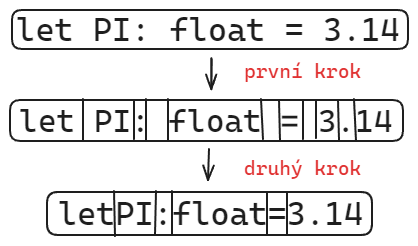
\includegraphics[width=0.5\linewidth]{image/lexer.png}
	\end{figure}
	
	\subsection{Syntaktická}
	
	Při syntaktické analýze dochází k parsování vstupních tokenů, hovoříme tak o parseru. Ten postupně prochází tokeny a vytváří z nich strukturu, určenou ke zpracování logickou částí.
	
	Pro Rudu jsem vytvořil vlastní univerzální parser. Používá programovatelný syntax čtený ze souboru, chybová hlášení generuje automaticky, a k tomu nabízí funkce pro debugování pravidel a jednoduchou validaci. Jeho syntax je jednoduchý a přehledný, programátor by měl být schopný zorientovat se už po pár minutách. Klíčové slovo let by v něm mohlo vypadat následovně:
	
	\begin{lstlisting}[caption={Ukázka klíčového slova let}]
	KWLet ident type expr
		"let" harderr="true"
		"'text" set="ident"
		: ?
			type ? set="type"
		= ?
			expr ? set="expr"
		; ?;
	\end{lstlisting}
	
	První řádek je hlavička slova začínající názvem „KWLet“ a pokračuje jeho parametry. Druhý porovnává, jestli je typ momentálního tokenu text s výrazem „let.“ Pokud ne, vrací error. Pokud ano, pokračuje dál a zapne harderr, ten říká, že pokud odteď dojde k chybě, tak není chybové pouze toto slovo, ale i jeho rodič, který dané slovo porovnával. Dále na řádku 3 porovnává jakýkoliv token reprezentující text. Pokud dojde ke schodě, nastaví parametr ident na porovnávaný token. Pokud nikoliv, vyhodí těžkou chybu (protože je zapnutý harderr). Otazník na řádku 4 znamená, že token není nutný. Pokud bude přítomen, vykoná se kód s vyšším odsazením (řádek č. 5). Středník na konci řádku 8 pouze oznamuje konec definice slova. Vytvořené slovo se později použije stejně jako na řádcích 5 a 7.
	
	Za zmínku stojí také metoda připojení zdrojových souborů. Kompilátor nemůže jen tak zpracovat všechny soubory s příponou .rd, co vidí. To by bylo náročné na zdroje počítače. Tento problém řeší tak, že nejprve získá vstupní soubor (mometálně pouze main.rd). Ten zpracuje a zapíše si použití klíčového slova import, které má cestu k použitému zdroji. Zatím si je pouze zapíše, protože kdyby je ihned zpracoval, tak může dojít k zamrznutí, při použití cyklických importů. Poté je zpracuje a označí jako zpracované.
	
	\clearpage
	
	
	\subsection{Sémantická}
	
	Poslední fáze analýzy má za úkol dát smysl struktuře získané po parsování. Protože parser je dynamický, tak musí nejprve vše vytáhnout do ucelené podoby a provést případné validace. Kontroluje například zda se neopakují názvy, ale také vytváří typy, parsuje matematické výrazy, apod.
	
	
	\section{Generace bytecode}
	
	Generace je nejdůležitější část každého překladače. Jde o proces, kdy zpracuje všechna získaná data a vytvoří užitečný produkt v podobě programu, či knihovny.
	
	Má implementace obsahuje generaci nejen bytecode, ale i informací pro debugování. To je užitečné v případě, že běžící Ruda program narazí na problém. Ruda VM díky toho zvládne podat důležité informace o původu problému.
	
	\subsection{Generace}
	
	Překladač před generací prošel třemi fázemi analýzi, aby měl znalost celého kódu. Samotná generace je ale stále velmi náročný proces. V kódu je obrovské množství způsobů, jak přistupovat k datům a jejich manipulaci. Transformace jazyk -> bytecode se potom stává velmi složitá, zmatečná a pokud provedení není perfektní, vytváří prostor pro nečekané chyby.
	
	Překladač začíná tím, že všem funkcím rozdá unikátní ID, které bude velmi důležité později. Vytvoří potřebné objekty společně s Ruda VM (pouze pro kompatibilitu; nikdy ho nespustí). Až bude vše připravené, začne s generací funkcí. Nezáleží na jejich pořadí, nakonec je zpracuje všechny.
	
	Pro překlad funkce používá rekurzivní prohledávání uzlů, které reprezentují výrazy. Pro každý vygeneruje patřičný bytecode. Například pro klíčové slovo let:
	
	\begin{lstlisting}[caption={Překlad klíčového slova let}]
	// vyraz
	let a = new 60
	
	// bytecode
	ReadConst(const_int_60, GENERAL_REG1)
	AllocateStatic(1)     
	WritePtr(GENERAL_REG1)   
	Write(a_stack_pos, POINTER_REG)  
	\end{lstlisting}
	
	Výraz vytvoří proměnnou a, do které zapíše ukazatel na hodnotu 60, která je uložená na haldě. Bytecode nejprve přečte hodnotu 60 z paměti a uloží ji do registru GENERAL-REG0. Potom na haldě vytvoří místo pro jednu hodnotu a ukazatel se automaticky uloží do registru POINTER-REG, který potom využije instrukce WritePtr, k tomu, aby na něj zapsala hodnotu z GENERAL-REG1, která je stále číslo 60. Už jenom potřebuje zapsat ukazatel, který stále přebývá v POINTER-REG do pozice na stacku vyhrazené pro proměnnou a.
	
	Tím tenhle příklad končí, ale je nutné vědět, že takhle bude bytecode vypadat až po optimalizaci. Generátor kódu je sám o sobě hloupí a nestará se o žádné stavy. Vždy zohledňuje pouze nejhorší možný případ a vytváří přitom poměrně nekvalitní a hlavně pomalý kód.
	
	\chapter{Virtuální stroj}
	
	V minulé kapitole jsme prošli, jak ze zdrojového kódu vznikne program. Zde se zaměříme na jeho spuštění pomocí Ruda VM, který je zodpovědný za provedení Ruda programů.
	
	
	\section{Instrukce}
	
	Instrukce jsou jedna ze částí Ruda bytecode. Jde o jednoduché pokyny, popisující co má provést Ruda VM. Jednotlivé instrukce jsou navrhnuté, pro co nejširší možné využití v rámci uzavřeného runtimu. 
	
	Právě proto lze Rudu použít tam, kde je bezpečnost priorita, pokud se povolí pouze moduly standardní knihovny pracující nezávisle na systému. Tato vlastnost by v budoucnu mohla Ruda běžet například na serverech, nebo jako skriptovací jazyk v jiném programu.
	
	Pro referenci jednotlivých instrukcí doporučuji prohlédnout přímo zdrojový kód runtimu, který lze nalézt na \url{https://github.com/it-2001/Ruda/blob/main/vm/runtime/src/lib.rs}. Zde můžete vyhledat "enum Instructions" (okolo řádku 2500), kde jsou všechny instrukce popsané.
	
	\section{Běh programu}
	
	Samotné jádro Rudy je pouze knihovna, nelze tudíž přímo spustit. K tomu pomáhá program Ruda VM, který zpracuje bytecode a připraví podle něj příslušné prostředí pro běh. Kromě toho podává zprávy o stavu, parsuje vstupní argumenty a připravuje potřebné knihovny.
	
	Poté, co Ruda VM připraví vše nutné, tak teprve spustí Ruda program. Instrukce běží sériově, dokud nenarazí na problém, nebo na konec programu označený instrukcí End.
	
	\clearpage
	\section{Model paměti}
	
	Pamět funguje na základě velmi využívané kombinace stacku, haldy a registrů. Pro většinu dat je tento způsob dostačující. Nedostatky se začnou ukazovat pokud chceme použít víc, než jen vlastní struktury. K pochopení tohoto problému je ale nutné vědět, jak Ruda ukládá data.
	
	Ruda je zároveň silně typovaný a dynamický jazyk. To znamená, že se typy kontrolují při kompilaci a zároveň za běhu programu. K tomu, aby typy mohly být otestovány dynamicky je nutné, aby každá hodnota obsahovala hlavičku udávající její typ. V případě ukazatelů nestačí pouze standardních 4 až 8 bytů z důvodů, které popíšu později a protože všechny typy musí mít schodnou velikost, tak každá hodnota zabírá přesně 24 bytů paměti.
	
	To by samo o sobě bylo v pořádku. Problém ale nastává při ukládání řetězců. Jeden řetězec s obsahem "Hello, world!" by měl zabrat 13 bytů. V Rudě vyroste ten stejný řetězec na celých 312 bytů. Tento nárust může být problematický zejména při zpracovávání velkých textů, jako jsou soubory, které mohou mnohonásobně nabýt na náročnosti pro paměť. Řešení bylo vytvořit novou haldu určenou pro řetězce. To umožňuje používat String typ v Rustu, který není jen rychlejší, ale přináší i užitečné vlastnosti jako kompatibilita s UTF-8 a celou škálu transformačních metod.
	
	Zbývalo ještě vyřešit, jak povolit nativním knihovnám ukládat vlastní data do Rudy. Tyto knihovny by mohly vytvořit objekt na haldě a vrátit ukazatel. Taková operace je ale náročná, protože vývojář knihovny musí zjistit, jak bude Ruda k takovému objektu přistupovat. Proto vznikla struktura podobná haldě, určená pro ukládání tzv. „user data“ - data neznámé velikosti, které splňují UserData interface. To dává Rudě schopnost vlastnit data, která by nešla uložit tradičnímy způsoby, jako například otevřené okno.
	
	\begin{figure}[h]
		\centering
		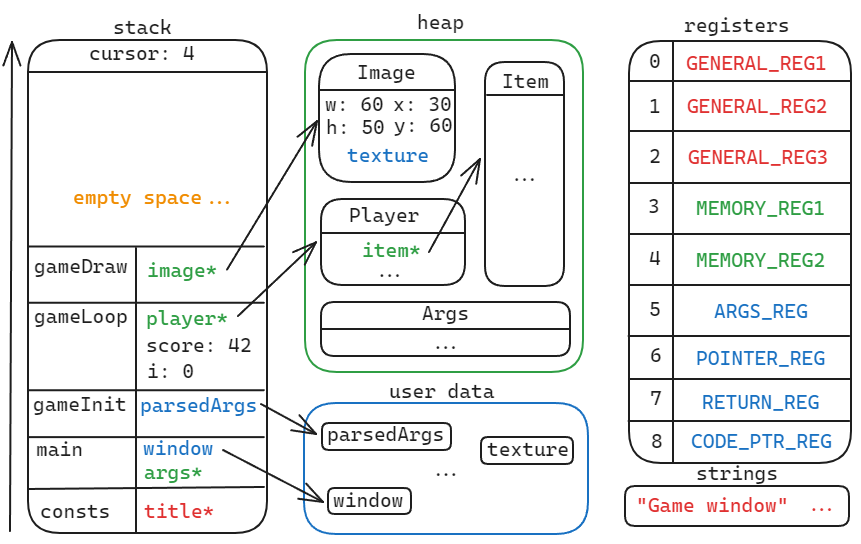
\includegraphics[width=0.8\linewidth]{image/memory.png}
	\end{figure}
	
	\section{Garbage collector}
	
	Všechny výše zmíněné struktury se musí čistit od nepoužívaných dat. Ruda proto nabízí vlastní garbage collector, fungující na principu dvou kroků.
	
	\subsection{Označení}
	
	První krok se nazívá označení. Jeho funkce je projít známou paměť a vyhledat všechna data, ke kterým se dostane pomocí existujících ukazatelů. Za známá data se považuje stack, registry a speciální struktura pro uložení argumentů funkcí. Pokud při označování nalezne ukazatel na haldu, řetězec, nebo user data, tak si zaznačí, že data můžou být stále použity. V případě, že zaznačí data na haldě, hledá nové ukazatele na dané pozici.
	
	\subsection{Úklid}
	
	Při úklidu najde všechna data, ke kterým není přístup na základě informací z první fáze a příslušné data uvolní pro další použití. Prostor zůstává přiřazený Ruda programu i po uvolnění, protože je velmi pravděpodobné, že pokud byl prostor použit jednou, tak bude znovu. Doporučuji proto periodicky spouštět úklid, aby bylo maximální využití paměti. Ruda nabízí modul pro manipulaci s garbage collectorem, takže si uživatel může vybrat vhodný čas.
	
	\section{Rozšíření pomocí nativních knihoven}
	
	Možnost pro nativní knihovny byla nevyhnutelná. Ruda nedovoluje žádný input ani output, takže program napsaný v čisté Rudě by byl zbytečný. Standardní knihovna proto používá veřejný interface pro Ruda nativní knihovny. 
	
	Tento interface může použít každý pro vlastní účely a rozšířit tak vlastnosti Rudy.
	
	Zatím pouze pro jazyk Rust.
	
	\section{Schopnost skriptování}
	
	Jedna z výhod toho, že Ruda runtime je pouze knihovna je, že lze použít jako skriptovací jazyk v jiném programu. Momentálně pro podobné využití nemá dostatečnou podporu, ale v budoucnu to bude standardní součást jazyka.
	
	\chapter{Nástroje pro práci s jazykem}
	
	Programování je jen část vývoje software. Důležité je také vývojové prostředí, přehlednost nástrojů a komunita vývojářů. Ruda jako začínající jazyk komunitu nemá, ale může se zaměřit na dva zbývající aspekty. Nabízí proto řadu nástrojů pro ulehčení vývojářského procesu.
	
	\section{Dokumentace}
	
	Žádnému jazyku nesmí chybět dokumentace. Pokud se povede správně, může být prvním místem, kde hledat pomoc. Dokumentace Rudy obsahuje vše, co by jakkoliv zkušený vývojář potřeboval. Výsvětluje témata začínající od instalace a prvního projektu, až po fungování paměti a ukáže Rudu v akci na projektech k vypracování.
	
	Dokumentace obsahuje i vlastnosti, které jsou v plánu do budoucna. Taková témata jsou vždy patřičně označeny.
	
	\section{Správce projektu}
	
	Integrovaný správce projektu zajišťuje snadnou práci s celkovým projektem. Mezi hlavní funkce patří vytvoření projektu, kompilace, spuštění a stažení knihoven ze vzdáleného git repozitáře. Stažené knihovny jsou uloženy do globální složky pro možnost opakovaného použití. Ruda jako nový jazyk žádné knihovny nemá, z tohoto důvodu nebyla jejich implementace příliš velkou prioritou a využití je tak zatím velmi omezené.
	
	Užitečná funkce pro kompilaci je uložení kontrolního řetězce, tento řetězec je vytvořen vždy při kompilaci. Pokud se vytvořený řetězec shoduje s tím minulým, tak správce předpokládá, že se obsah projektu nezměnil a přeskočí kompilaci.
	
	\clearpage
	
	\section{Standardní knihovna}
	
	Standardní knihovna je zaměřená hlavně na funkce, které v čisté Rudě nelze napsat. 
	Mezi ně patří například.
	
	\begin{enumerate}
		\item Systém - práce se souborovým systémem počítače, parametry programu, systémový čas a funkce pro vstup a výstup.
		\item Paměť - správa paměti runtimu. Slouží primárně jako abstrakce pro garbage collector.
		\item Metody typů - obsahuje také některé metody pro vnitřní typy včetně čísel, polí a řetězců.
		\item Okno - Pro snadný vývoj aplikací je zde obsažen i modul pro práci s okny. Ten využívá SFML pro fungovaní okna, ale má vlastní elegantní implementaci.
	\end{enumerate}
	
	\section{Grafický inspektor Ruda projektu}
	
	Interaktivní program Ruda lens je určený jako doplněk ručně psané dokumentace. Po spuštění příkazu ruda lens se otevře aplikace s přehledem projektu. Obsahuje náhled všech deklarací. Příkaz ruda lens -t bin je experimentální funkce s přehledem Ruda bytecode.
	
	\begin{figure}[h]
		\centering
		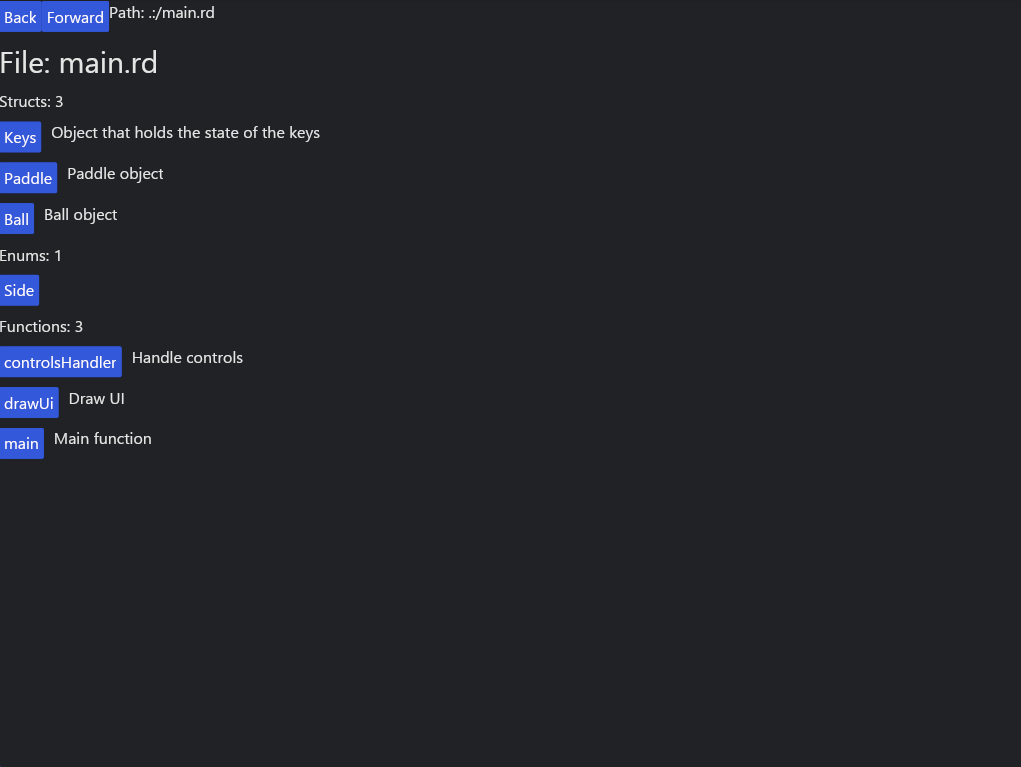
\includegraphics[width=0.8\linewidth]{image/lens.png}
	\end{figure}
	
	\section{Syntax highlighting}
	
	Existuje také rozšíření pro textový editor Visual studio code. Poskytuje vylepšený syntax highlighting. Jedná se pouze o zbarvení kódu, LSP (language server protocol) není implementované. Budoucí implementace LSP by fungovala podobně jako Ruda lens.
	
	\chapter{Instalace}
	
	Krátká kapitola o instalaci Rudy. Celá instalace je popsaná i v hlavním repozitáři.
	
	\section{Podporované platformy}
	
	Zatím pouze 64 bitový windows. Hlavní příčina je kompilace Rust projektu s SFML na Linuxu. V budoucnu bude problém vyřešen a přidám širší podporu platforem.
	
	\section{Stažení}
	
	Hlavní repozitář obsahuje verzi v0.1.0-alpha, zde jsou potřebné binárky v zip souboru a testovací program.
	
	\subsection{Kompilace ze zdrojových kódů}
	
	Vyžaduje předem nainstalovat:
	
	\begin{enumerate}
		\item Python
		\item Rust
		\item SFML - včetně vytvoření potřebných proměnných prostředí.
	\end{enumerate}
	
	Dále naklonovat hlavní repozitář. Pokud se vše povedlo, stačí spustit python skript ruda\_build.py a vytvoří se složka s názvem build.
	
	\section{Proměnné prostředí}
	
	Ruda vyžeduje 2 proměnné:
	
	\begin{enumerate}
		\item Path - do proměnné path přidat cestu do složky build/bin.
		\item Ruda root - vytvořit proměnnou RUDA\_PATH a nastavit ji na cestu do složky build.
	\end{enumerate}
	
	\chapter{Programování v Rudě}
	
	Toto téma je do hloubky vysvětleno v oficiální dokumentaci, takže tady pouze projdu některé zajímavosti. Dokumentaci lze najít na: \url{https://it-2001.github.io/Ruda-docs/}
	
	\section{Syntaxe}
	
	Ruda je C-like programovací jazyk. To znamená, že se podobá většině moderních jazyků a přechod na Rudu je proto mnohem snažší. Změna oproti ostatním jazykům je psaní objektů. Pro deklaraci používá klíčové slovo struct, ale při vytváření instancí stále vyžaduje využití konstruktoru.
	
	\begin{lstlisting}[caption={Struktura}]
	struct Auto {
		rychlost: float
		barva_: Color
		
		new (barva: Color) {
			self.barva_ = barva
			self.rychlost = 210
		}
		
		fun barva(self, barva: Color?): Color {
			if barva? {
				self.barva_ = barva
			}
			return self.barva_
		}
	}
	\end{lstlisting}
	
	\clearpage
	
	Výjimky mají vlastní klíčové slovo error a speciální syntax. To z důvodu, že výjimky můžou být časté, i když je kód ignoruje. Speciální syntax umožňuje vytvářet líné výjimky, které nezdržují program, pokud jsou zahozeny.
	
	\begin{lstlisting}[caption={Výjimky}]
	error Error(message: string?) {
		message: {
			if message? {
				return message
			} else {
				return "Neco se pokazilo"
			}
		}
		code: 1,
	}
	\end{lstlisting}
	
	\chapter*{Závěr}
	
	\addcontentsline{toc}{chapter}{Závěr}
	
	Ruda je můj doposud největší projekt. Kombinuje mnoho různých odvětví programování, s většinou z nich jsem se při vývoji setkal poprvé. Projekt sice nemá moc komerční hodnotu vzhledem k tomu, že existují mraky skvělých jazyků a jejich knihoven, zato ale mě osobně dal hodnotné zkušenosti a úctu k nástrojům, které dnes existují.
	
	Většinu věcí jsem dělal sám bez zdrojů z internetu, takže se moje řešení možná bude lišit od těch komerčních. Až potom, co jsem dokončil nějakou část jazyka, jsem se podíval, jak to řeší ostatní.
	
	\section*{Splněné cíle}
	
	Jazyk je použitelný a vestavěné nástroje dokážou opravdu zpříjemnit jeho používání. Podle toho si mýslím, že hlavní cíle jsem splnil. Dále mě ale čeká dodělání některých funkcí, polishing, opravení chyb a rozšíření standardní knihovny.
	
	\section*{Poznatky}
	
	Při psaní kompilátoru mi hodně pomohl jazyk Rust, ve kterém jsem vše psal. Když jsem ale psal runtime, tak i když mi Rust zase velmi pomáhal, tak si začínám uvědomovat, že pro takový program by bylo lepší použít jazyk s větší kontrolou nad paměcí, jako je C nebo Zig. Rust vyžaduje ověření správnosti za běhu programu, což se stává zbytečné, když úkol runtimu je zpracovat bytecode, který je zaručeně správný. To způsobuje značnou ztrátu výkonu.
	
	\section*{Možnosti dalšího vývoje}
	
	Chtěl bych udělat snadnou podporu pro skriptování. V dnešní době existuje jen pár jazyků s dobrou podporou pro skriptování a přidání takového jazyku často vyžaduje zvláštní postupy. Jediný moderní jazyk, který do těchto kritérií zapadá je Lua, ta ale přináší výkonové nedostatky a snadný syntax může být často přínosem, ale rozhodně se nedá považovat za univerzální řešení.
	
	
	%% literatura
	\renewcommand\bibname{Použité zdroje informací}
	\begin{thebibliography}{99}
		
		\bibitem{GC} Microsoft [online]. Fundamentals of garbage collection. Microsoft. 2023 [cit. 2024-04-11]. Dostupné z: \url{https://learn.microsoft.com/en-us/dotnet/standard/garbage-collection/fundamentals}.
		\bibitem{VM} Robert Nystrom. Crafting interpreters. [online]. 2023 [cit. 2023-04-11] Dostupné z: \url{https://craftinginterpreters.com/}.
		\bibitem{Tsoding} Tsoding daily. Playlist videí o vývoji jazyka Porth. Https://www.youtube.com/ [online]. 2023 [cit. 2023-04-11]. Dostupné z: \url{https://www.youtube.com/watch?v=8QP2fDBIxjM&list=PLpM-Dvs8t0VbMZA7wW9aR3EtBqe2kinu4}.
		\bibitem{Rust} Rust [online]. The Rust Programming Language. 2023 [cit. 2023-11-4].  Dostupné z: \url{https://doc.rust-lang.org/book/}.
		
		
	\end{thebibliography}
	
		
	\appendix %% začínají přílohy
		
	\titleformat{\chapter}[block]{\scshape\bfseries\LARGE}{Příloha \thechapter}{10pt}{\vspace{0pt}}[\vspace{-22pt}] %% nastavení nadpisu u příloh
		
	
		
	
\end{document}
